% Options for packages loaded elsewhere
\PassOptionsToPackage{unicode}{hyperref}
\PassOptionsToPackage{hyphens}{url}
%
\documentclass[
  12pt,
  a4paper,
  twoside]{book}
\usepackage{amsmath,amssymb}
\usepackage{lmodern}
\usepackage{setspace}
\usepackage{ifxetex,ifluatex}
\ifnum 0\ifxetex 1\fi\ifluatex 1\fi=0 % if pdftex
  \usepackage[T1]{fontenc}
  \usepackage[utf8]{inputenc}
  \usepackage{textcomp} % provide euro and other symbols
\else % if luatex or xetex
  \usepackage{unicode-math}
  \defaultfontfeatures{Scale=MatchLowercase}
  \defaultfontfeatures[\rmfamily]{Ligatures=TeX,Scale=1}
  \setmainfont[]{Times New Roman}
  \setsansfont[]{Arial}
\fi
% Use upquote if available, for straight quotes in verbatim environments
\IfFileExists{upquote.sty}{\usepackage{upquote}}{}
\IfFileExists{microtype.sty}{% use microtype if available
  \usepackage[]{microtype}
  \UseMicrotypeSet[protrusion]{basicmath} % disable protrusion for tt fonts
}{}
\makeatletter
\@ifundefined{KOMAClassName}{% if non-KOMA class
  \IfFileExists{parskip.sty}{%
    \usepackage{parskip}
  }{% else
    \setlength{\parindent}{0pt}
    \setlength{\parskip}{6pt plus 2pt minus 1pt}}
}{% if KOMA class
  \KOMAoptions{parskip=half}}
\makeatother
\usepackage{xcolor}
\IfFileExists{xurl.sty}{\usepackage{xurl}}{} % add URL line breaks if available
\IfFileExists{bookmark.sty}{\usepackage{bookmark}}{\usepackage{hyperref}}
\hypersetup{
  pdftitle={Biomedical Knowledge Mining using GOSemSim and clusterProfiler},
  pdfauthor={Guangchuang Yu},
  hidelinks,
  pdfcreator={LaTeX via pandoc}}
\urlstyle{same} % disable monospaced font for URLs
\usepackage[left=35mm,right=35mm,top=25mm,bottom=25mm]{geometry}
\usepackage{color}
\usepackage{fancyvrb}
\newcommand{\VerbBar}{|}
\newcommand{\VERB}{\Verb[commandchars=\\\{\}]}
\DefineVerbatimEnvironment{Highlighting}{Verbatim}{commandchars=\\\{\}}
% Add ',fontsize=\small' for more characters per line
\usepackage{framed}
\definecolor{shadecolor}{RGB}{248,248,248}
\newenvironment{Shaded}{\begin{snugshade}}{\end{snugshade}}
\newcommand{\AlertTok}[1]{\textcolor[rgb]{0.94,0.16,0.16}{#1}}
\newcommand{\AnnotationTok}[1]{\textcolor[rgb]{0.56,0.35,0.01}{\textbf{\textit{#1}}}}
\newcommand{\AttributeTok}[1]{\textcolor[rgb]{0.77,0.63,0.00}{#1}}
\newcommand{\BaseNTok}[1]{\textcolor[rgb]{0.00,0.00,0.81}{#1}}
\newcommand{\BuiltInTok}[1]{#1}
\newcommand{\CharTok}[1]{\textcolor[rgb]{0.31,0.60,0.02}{#1}}
\newcommand{\CommentTok}[1]{\textcolor[rgb]{0.56,0.35,0.01}{\textit{#1}}}
\newcommand{\CommentVarTok}[1]{\textcolor[rgb]{0.56,0.35,0.01}{\textbf{\textit{#1}}}}
\newcommand{\ConstantTok}[1]{\textcolor[rgb]{0.00,0.00,0.00}{#1}}
\newcommand{\ControlFlowTok}[1]{\textcolor[rgb]{0.13,0.29,0.53}{\textbf{#1}}}
\newcommand{\DataTypeTok}[1]{\textcolor[rgb]{0.13,0.29,0.53}{#1}}
\newcommand{\DecValTok}[1]{\textcolor[rgb]{0.00,0.00,0.81}{#1}}
\newcommand{\DocumentationTok}[1]{\textcolor[rgb]{0.56,0.35,0.01}{\textbf{\textit{#1}}}}
\newcommand{\ErrorTok}[1]{\textcolor[rgb]{0.64,0.00,0.00}{\textbf{#1}}}
\newcommand{\ExtensionTok}[1]{#1}
\newcommand{\FloatTok}[1]{\textcolor[rgb]{0.00,0.00,0.81}{#1}}
\newcommand{\FunctionTok}[1]{\textcolor[rgb]{0.00,0.00,0.00}{#1}}
\newcommand{\ImportTok}[1]{#1}
\newcommand{\InformationTok}[1]{\textcolor[rgb]{0.56,0.35,0.01}{\textbf{\textit{#1}}}}
\newcommand{\KeywordTok}[1]{\textcolor[rgb]{0.13,0.29,0.53}{\textbf{#1}}}
\newcommand{\NormalTok}[1]{#1}
\newcommand{\OperatorTok}[1]{\textcolor[rgb]{0.81,0.36,0.00}{\textbf{#1}}}
\newcommand{\OtherTok}[1]{\textcolor[rgb]{0.56,0.35,0.01}{#1}}
\newcommand{\PreprocessorTok}[1]{\textcolor[rgb]{0.56,0.35,0.01}{\textit{#1}}}
\newcommand{\RegionMarkerTok}[1]{#1}
\newcommand{\SpecialCharTok}[1]{\textcolor[rgb]{0.00,0.00,0.00}{#1}}
\newcommand{\SpecialStringTok}[1]{\textcolor[rgb]{0.31,0.60,0.02}{#1}}
\newcommand{\StringTok}[1]{\textcolor[rgb]{0.31,0.60,0.02}{#1}}
\newcommand{\VariableTok}[1]{\textcolor[rgb]{0.00,0.00,0.00}{#1}}
\newcommand{\VerbatimStringTok}[1]{\textcolor[rgb]{0.31,0.60,0.02}{#1}}
\newcommand{\WarningTok}[1]{\textcolor[rgb]{0.56,0.35,0.01}{\textbf{\textit{#1}}}}
\usepackage{longtable,booktabs,array}
\usepackage{calc} % for calculating minipage widths
% Correct order of tables after \paragraph or \subparagraph
\usepackage{etoolbox}
\makeatletter
\patchcmd\longtable{\par}{\if@noskipsec\mbox{}\fi\par}{}{}
\makeatother
% Allow footnotes in longtable head/foot
\IfFileExists{footnotehyper.sty}{\usepackage{footnotehyper}}{\usepackage{footnote}}
\makesavenoteenv{longtable}
\usepackage{graphicx}
\makeatletter
\def\maxwidth{\ifdim\Gin@nat@width>\linewidth\linewidth\else\Gin@nat@width\fi}
\def\maxheight{\ifdim\Gin@nat@height>\textheight\textheight\else\Gin@nat@height\fi}
\makeatother
% Scale images if necessary, so that they will not overflow the page
% margins by default, and it is still possible to overwrite the defaults
% using explicit options in \includegraphics[width, height, ...]{}
\setkeys{Gin}{width=\maxwidth,height=\maxheight,keepaspectratio}
% Set default figure placement to htbp
\makeatletter
\def\fps@figure{htbp}
\makeatother
\setlength{\emergencystretch}{3em} % prevent overfull lines
\providecommand{\tightlist}{%
  \setlength{\itemsep}{0pt}\setlength{\parskip}{0pt}}
\setcounter{secnumdepth}{5}
\ifluatex
  \usepackage{selnolig}  % disable illegal ligatures
\fi
\newlength{\cslhangindent}
\setlength{\cslhangindent}{1.5em}
\newlength{\csllabelwidth}
\setlength{\csllabelwidth}{3em}
\newenvironment{CSLReferences}[2] % #1 hanging-ident, #2 entry spacing
 {% don't indent paragraphs
  \setlength{\parindent}{0pt}
  % turn on hanging indent if param 1 is 1
  \ifodd #1 \everypar{\setlength{\hangindent}{\cslhangindent}}\ignorespaces\fi
  % set entry spacing
  \ifnum #2 > 0
  \setlength{\parskip}{#2\baselineskip}
  \fi
 }%
 {}
\usepackage{calc}
\newcommand{\CSLBlock}[1]{#1\hfill\break}
\newcommand{\CSLLeftMargin}[1]{\parbox[t]{\csllabelwidth}{#1}}
\newcommand{\CSLRightInline}[1]{\parbox[t]{\linewidth - \csllabelwidth}{#1}\break}
\newcommand{\CSLIndent}[1]{\hspace{\cslhangindent}#1}

\title{Biomedical Knowledge Mining using GOSemSim and clusterProfiler}
\author{Guangchuang Yu}
\date{2021-07-21}

\begin{document}
\maketitle

{
\setcounter{tocdepth}{2}
\tableofcontents
}
\setstretch{1.5}
\hypertarget{introduction}{%
\chapter*{📖 Introduction}\label{introduction}}
\addcontentsline{toc}{chapter}{📖 Introduction}

\href{https://github.com/YuLab-SMU/ChIPseeker}{\includegraphics{https://img.shields.io/badge/ChIPseeker-1.28.3-green.svg}}
\href{https://github.com/YuLab-SMU/clusterProfiler}{\includegraphics{https://img.shields.io/badge/clusterProfiler-4.0.2-green.svg}}
\href{https://github.com/YuLab-SMU/DOSE}{\includegraphics{https://img.shields.io/badge/DOSE-3.18.1-green.svg}}
\href{https://github.com/YuLab-SMU/enrichplot}{\includegraphics{https://img.shields.io/badge/enrichplot-1.12.2-green.svg}}
\href{https://github.com/YuLab-SMU/GOSemSim}{\includegraphics{https://img.shields.io/badge/GOSemSim-2.18.0-green.svg}}
\href{https://github.com/YuLab-SMU/meshes}{\includegraphics{https://img.shields.io/badge/meshes-1.18.0-green.svg}}
\href{https://github.com/YuLab-SMU/ReactomePA}{\includegraphics{https://img.shields.io/badge/ReactomePA-1.36.0-green.svg}}

\hypertarget{motivation}{%
\section*{🎯 Motivation}\label{motivation}}
\addcontentsline{toc}{section}{🎯 Motivation}

The book is meant as a guide for mining biological knowledge to elucidate or interpret molecular mechanisms using a suite of R packages, including \href{http://bioconductor.org/packages/ChIPseeker}{ChIPseeker}, \href{http://bioconductor.org/packages/clusterProfiler}{clusterProfiler}, \href{http://bioconductor.org/packages/DOSE}{DOSE}, \href{http://bioconductor.org/packages/enrichplot}{enrichplot}, \href{http://bioconductor.org/packages/GOSemSim}{GOSemSim}, \href{http://bioconductor.org/packages/meshes}{meshes} and \href{http://bioconductor.org/packages/ReactomePA}{ReactomePA}. Hence, if you are starting to read this book, we assume you have a working knowledge of how to use R.

\hypertarget{citation}{%
\section*{📝 Citation}\label{citation}}
\addcontentsline{toc}{section}{📝 Citation}

If you use the software suite in published research, please cite the most appropriate paper(s) from this list:

\begin{enumerate}
\def\labelenumi{\arabic{enumi}.}
\tightlist
\item
  T Wu\#, E Hu\#, S Xu, M Chen, P Guo, Z Dai, T Feng, L Zhou, W Tang, L Zhan, X Fu, S Liu, X Bo*, and \textbf{G Yu}*. clusterProfiler 4.0: A universal enrichment tool for interpreting omics data. \textbf{\emph{The Innovation}}. 2021, accepted.
  doi: \href{https://doi.org/10.1016/j.xinn.2021.100141}{10.1016/j.xinn.2021.100141}
\item
  \textbf{G Yu}\textsuperscript{*}. Gene Ontology Semantic Similarity Analysis Using GOSemSim. In: Kidder B. (eds) Stem Cell Transcriptional Networks. \textbf{\emph{Methods in Molecular Biology}}. 2020, 2117:207-215. Humana, New York, NY.
  doi: \href{https://doi.org/10.1007/978-1-0716-0301-7_11}{10.1007/978-1-0716-0301-7\_11}
\item
  \textbf{G Yu}\textsuperscript{*}. Using meshes for MeSH term enrichment and semantic analyses. \textbf{\emph{Bioinformatics}}. 2018, 34(21):3766--3767.
  doi: \href{https://doi.org/10.1093/bioinformatics/bty410}{10.1093/bioinformatics/bty410}
\item
  \textbf{G Yu}, QY He\textsuperscript{*}. ReactomePA: an R/Bioconductor package for reactome pathway analysis and visualization. \textbf{\emph{Molecular BioSystems}}. 2016, 12(2):477-479.
  doi: \href{https://doi.org/10.1039/C5MB00663E}{10.1039/C5MB00663E}
\item
  \textbf{G Yu}\textsuperscript{*}, LG Wang, and QY He\textsuperscript{*}. ChIPseeker: an R/Bioconductor package for ChIP peak annotation, comparison and visualization. \textbf{\emph{Bioinformatics}}. 2015, 31(14):2382-2383.
  doi: \href{https://doi.org/10.1093/bioinformatics/btv145}{10.1093/bioinformatics/btv145}
\item
  \textbf{G Yu}\textsuperscript{*}, LG Wang, GR Yan, QY He\textsuperscript{*}. DOSE: an R/Bioconductor package for Disease Ontology Semantic and Enrichment analysis. \textbf{\emph{Bioinformatics}}. 2015, 31(4):608-609.
  doi: \href{https://doi.org/10.1093/bioinformatics/btu684}{10.1093/bioinformatics/btu684}
\item
  \textbf{G Yu}, LG Wang, Y Han and QY He\textsuperscript{*}. clusterProfiler: an R package for comparing biological themes among gene clusters. \textbf{\emph{OMICS: A Journal of Integrative Biology}}. 2012, 16(5):284-287.
  doi: \href{https://doi.org/10.1089/omi.2011.0118}{10.1089/omi.2011.0118}
\item
  \textbf{G Yu}, F Li, Y Qin, X Bo\textsuperscript{*}, Y Wu, S Wang\textsuperscript{*}. GOSemSim: an R package for measuring semantic similarity among GO terms and gene products. \textbf{\emph{Bioinformatics}}. 2010, 26(7):976-978.
  doi: \href{https://doi.org/10.1093/bioinformatics/btq064}{10.1093/bioinformatics/btq064}
\end{enumerate}

\hypertarget{book-structure}{%
\section*{📚 Book structure}\label{book-structure}}
\addcontentsline{toc}{section}{📚 Book structure}

\begin{itemize}
\tightlist
\item
  Part 1 (Semantic similarity analysis) describes \href{http://bioconductor.org/packages/GOSemSim}{GOSemSim}, \href{http://bioconductor.org/packages/DOSE}{DOSE} and \href{http://bioconductor.org/packages/meshes}{meshes} packages for measuring semantic similarity of genes or gene products based on Gene Ontology, Disease Ontology and Medical Subject Headings.
\item
  Part 2 (Enrichment analysis) introduces over-reprensentation analysis and gene set enrichment analysis using \href{http://bioconductor.org/packages/clusterProfiler}{clusterProfiler} (supports GO, KEGG, MSigDb, WikiPathway, and many others via universal interface), \href{http://bioconductor.org/packages/DOSE}{DOSE} (DO, Disease-Gene Network, Network of Cancer Genes), \href{http://bioconductor.org/packages/meshes}{meshes} (MeSH), and \href{http://bioconductor.org/packages/ReactomePA}{ReactomePA} (Reactome pathway). Functional enrichment analysis of Genomic coordination is supported via \href{http://bioconductor.org/packages/ChIPseeker}{ChIPseeker} and comparison among multiple conditions is also supported by \href{http://bioconductor.org/packages/clusterProfiler}{clusterProfiler}. We implemented a number of visualization methods in the \href{http://bioconductor.org/packages/enrichplot}{enrichplot} package to help users to interpret their results.
\item
  Part 3 (Miscellaneous topics) describes useful utilities including translating gene IDs and manipulating enrichment results.
\end{itemize}

\hypertarget{want-to-help}{%
\section*{💖 Want to help?}\label{want-to-help}}
\addcontentsline{toc}{section}{💖 Want to help?}

The book's source code is hosted on GitHub, at \url{https://github.com/YuLab-SMU/biomedical-knowledge-mining-book}. Any feedback on the book is very welcome. Feel free to \href{https://github.com/YuLab-SMU/biomedical-knowledge-mining-book/issues/new}{open an issue} on GitHub or send me a pull request if you notice typos or other issues (I'm not a native English speaker ;) ).

\hypertarget{intro}{%
\chapter{Introduction}\label{intro}}

You can label chapter and section titles using \texttt{\{\#label\}} after them, e.g., we can reference Chapter \ref{intro}. If you do not manually label them, there will be automatic labels anyway, e.g., Chapter \ref{methods}.

Figures and tables with captions will be placed in \texttt{figure} and \texttt{table} environments, respectively.

\begin{Shaded}
\begin{Highlighting}[]
\FunctionTok{par}\NormalTok{(}\AttributeTok{mar =} \FunctionTok{c}\NormalTok{(}\DecValTok{4}\NormalTok{, }\DecValTok{4}\NormalTok{, .}\DecValTok{1}\NormalTok{, .}\DecValTok{1}\NormalTok{))}
\FunctionTok{plot}\NormalTok{(pressure, }\AttributeTok{type =} \StringTok{\textquotesingle{}b\textquotesingle{}}\NormalTok{, }\AttributeTok{pch =} \DecValTok{19}\NormalTok{)}
\end{Highlighting}
\end{Shaded}

\begin{figure}

{\centering 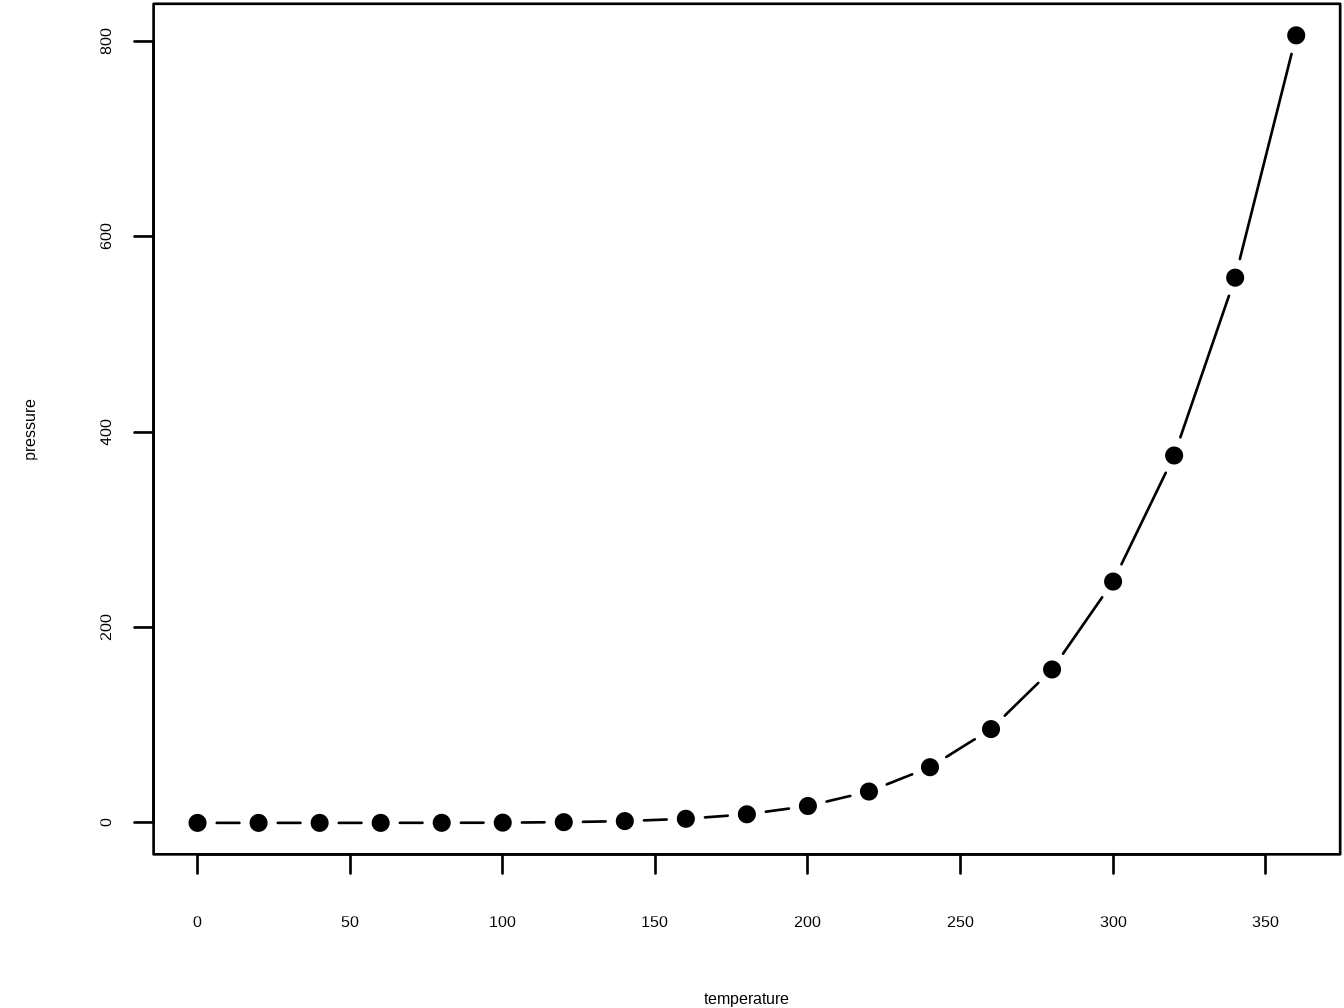
\includegraphics[width=0.8\linewidth]{sigminer_files/figure-latex/nice-fig-1} 

}

\caption{Here is a nice figure!}\label{fig:nice-fig}
\end{figure}

Reference a figure by its code chunk label with the \texttt{fig:} prefix, e.g., see Figure \ref{fig:nice-fig}. Similarly, you can reference tables generated from \texttt{knitr::kable()}, e.g., see Table \ref{tab:nice-tab}.

\begin{Shaded}
\begin{Highlighting}[]
\NormalTok{knitr}\SpecialCharTok{::}\FunctionTok{kable}\NormalTok{(}
  \FunctionTok{head}\NormalTok{(iris, }\DecValTok{20}\NormalTok{), }\AttributeTok{caption =} \StringTok{\textquotesingle{}Here is a nice table!\textquotesingle{}}\NormalTok{,}
  \AttributeTok{booktabs =} \ConstantTok{TRUE}
\NormalTok{)}
\end{Highlighting}
\end{Shaded}

\begin{table}

\caption{\label{tab:nice-tab}Here is a nice table!}
\centering
\begin{tabular}[t]{rrrrl}
\toprule
Sepal.Length & Sepal.Width & Petal.Length & Petal.Width & Species\\
\midrule
5.1 & 3.5 & 1.4 & 0.2 & setosa\\
4.9 & 3.0 & 1.4 & 0.2 & setosa\\
4.7 & 3.2 & 1.3 & 0.2 & setosa\\
4.6 & 3.1 & 1.5 & 0.2 & setosa\\
5.0 & 3.6 & 1.4 & 0.2 & setosa\\
\addlinespace
5.4 & 3.9 & 1.7 & 0.4 & setosa\\
4.6 & 3.4 & 1.4 & 0.3 & setosa\\
5.0 & 3.4 & 1.5 & 0.2 & setosa\\
4.4 & 2.9 & 1.4 & 0.2 & setosa\\
4.9 & 3.1 & 1.5 & 0.1 & setosa\\
\addlinespace
5.4 & 3.7 & 1.5 & 0.2 & setosa\\
4.8 & 3.4 & 1.6 & 0.2 & setosa\\
4.8 & 3.0 & 1.4 & 0.1 & setosa\\
4.3 & 3.0 & 1.1 & 0.1 & setosa\\
5.8 & 4.0 & 1.2 & 0.2 & setosa\\
\addlinespace
5.7 & 4.4 & 1.5 & 0.4 & setosa\\
5.4 & 3.9 & 1.3 & 0.4 & setosa\\
5.1 & 3.5 & 1.4 & 0.3 & setosa\\
5.7 & 3.8 & 1.7 & 0.3 & setosa\\
5.1 & 3.8 & 1.5 & 0.3 & setosa\\
\bottomrule
\end{tabular}
\end{table}

You can write citations, too. For example, we are using the \textbf{bookdown} package (\protect\hyperlink{ref-R-bookdown}{\textbf{R-bookdown?}}) in this sample book, which was built on top of R Markdown and \textbf{knitr} (\protect\hyperlink{ref-xie2015}{Xie 2015}).

\hypertarget{literature}{%
\chapter{Literature}\label{literature}}

Here is a review of existing methods.

\hypertarget{methods}{%
\chapter{Methods}\label{methods}}

We describe our methods in this chapter.

\hypertarget{applications}{%
\chapter{Applications}\label{applications}}

Some \emph{significant} applications are demonstrated in this chapter.

\hypertarget{example-one}{%
\section{Example one}\label{example-one}}

\hypertarget{example-two}{%
\section{Example two}\label{example-two}}

\hypertarget{final-words}{%
\chapter{Final Words}\label{final-words}}

We have finished a nice book.

\hypertarget{refs}{}
\begin{CSLReferences}{1}{0}
\leavevmode\hypertarget{ref-xie2015}{}%
Xie, Yihui. 2015. \emph{Dynamic Documents with {R} and Knitr}. 2nd ed. Boca Raton, Florida: Chapman; Hall/CRC. \url{http://yihui.org/knitr/}.

\end{CSLReferences}

\end{document}
